\documentclass[submission]{gmp2017}
%\documentclass{gmp2017}

\title{Parallel Quadtree Construction on Collections of Objects}

% Put your submission number here.
% This number will appear instead of authors and affiliations if the
% class option "submission" is active.
\SubNumber{142}

% Put the author names here.
% Use the second argument as a reference to the list of affiliations.
% No authors and affiliations will appear if the class option "submission"
% is active.
\author{John Edwards}{1}
\author{Nathan Vollmer}{1}
\author{Nicholas Harrison}{1}

% Put the affiliations of the authors here.
\affiliation{1}{Department of Informatics and Computer Science, Idaho State University, USA}

%\usepackage{amsmath,amsthm,amsfonts,amscd,amssymb,amstext} 
\usepackage{amsmath,amsfonts,amscd,amssymb,amstext} 
\usepackage{mathrsfs}
				% Some packages to write mathematics.
\usepackage{overpic}
\usepackage{eucal} 	 	% Euler fonts
\usepackage{verbatim}      	% Allows quoting source with commands.
\usepackage{makeidx}       	% Package to make an index.
%\usepackage{citesort}         	% 
\usepackage{subfig}
\usepackage{graphicx}
\usepackage{url}		% Allows good typesetting of web URLs.
\usepackage{multirow}
%\usepackage[linesnumbered, noline]{algorithm2e}
%\usepackage[boxed, noline]{algorithm2e}
\usepackage[ruled]{algorithm2e}
\usepackage{booktabs}
\usepackage{tabularx}
\usepackage{array}
\usepackage{adjustbox}
\usepackage{color}
\usepackage{tikz}
% To balance the columns at the end
\usepackage{balance}
\usepackage[mediumspace,mediumqspace,Grey,squaren]{SIunits}
%\usepackage{draftcopy}		% Uncomment this line to have the
				% word, "DRAFT," as a background
				% "watermark" on all of the pages of
				% of your draft versions. When ready
				% to generate your final copy, re-comment
				% it out with a percent sign to remove
				% the word draft before you re-run
				% Makediss for the last time.
\usepackage[normalem]{ulem}

%\usepackage{cite}
\usepackage{balance}
\usepackage{color}

\definecolor{bostonuniversityred}{rgb}{0.8, 0.0, 0.0}
\definecolor{medblue}{rgb}{0.0, 0.0, 0.7}

%------------------------------------------------------------
% Custom commands
%------------------------------------------------------------
%\newcommand{\old}[1]{\textcolor{blue}{\sout{#1}}}
\newcommand{\old}[1]{}

%\newcommand{\red}[1]{\textcolor{red}{#1}}
\newcommand{\red}[1]{\textcolor{bostonuniversityred}{#1}}
\newcommand{\blue}[1]{\textcolor{medblue}{#1}}
\definecolor{light-gray}{gray}{0.75}
\newcommand{\gray}[1]{\textcolor{light-gray}{#1}}
%\newcommand{\red}[1]{#1}

%\newcommand{\reconstruct}{RECONSTRUCT\textsuperscript{\texttrademark}}
%\newcommand{\tm}{\textsuperscript{\texttrademark}}
\newcommand{\tm}{$^1$}
\newcommand{\addref}{\red{REF}}
\newcommand{\mathtext}[1]{\text{#1}}
\newcommand{\etal}{et al.\ }
\newcommand{\algorithmspace}{\vspace{8pt}}
\newcommand{\glfs}{\emph{glfs}}

\renewcommand{\vec}[1]{\mathbf{#1}}

\newcommand{\centercell}[1]{\multicolumn{1}{c}{#1}}
\newcolumntype{x}[1]{>{\centering\arraybackslash\hspace{0pt}}m{#1}}
\newcolumntype{y}[1]{>{\centering\arraybackslash\hspace{0pt}}m{#1\textwidth}}
\newcolumntype{M}{>{\centering\arraybackslash}m{1cm}}

\DeclareMathOperator*{\argmin}{arg\,min}
\DeclareMathOperator*{\argmax}{arg\,max}

\newcommand{\BigO}[1]{\ensuremath{\operatorname{O}\left(#1\right)}}
\newcommand{\centroid}{\mathscr{C}}
\newcommand{\iring}{\mathscr{R}}

% aligned
\renewcommand{\d}{\delta}
\newcommand{\vempty}{\mathscr{E}}
\newcommand{\e}{\epsilon}
\newcommand{\dist}{\mathtext{dist}}
\newcommand{\ball}{\mathscr{B}}


\newcommand{\hgt}{22mm}

%%--------------------------------------------------
%% Theorem environments (amsthm package required)
%%--------------------------------------------------
%% \theoremstyle{plain} %% This is the default
%\newtheorem{theorem}{Theorem}
%\newtheorem{lemma}{Lemma}
%\newtheorem{corollary}{Corollary}
%\newtheorem{conjecture}{Conjecture}
%\newtheorem{crit}{Criterion}
%\newtheorem{condition}{Condition}
%\newtheorem{fact}{Fact}

%\theoremstyle{definition}
%\newtheorem{defn}{Definition}[section]

%\theoremstyle{remark}
%\newtheorem{rem}{Remark}[section]
%\newtheorem*{notation}{Notation}

%\numberwithin{equation}{section}

%--------------------------------------------------
% Tight enumerations
%--------------------------------------------------
\newenvironment{tightenumerate}{
\begin{enumerate}
  \setlength{\itemsep}{1pt}
  \setlength{\parskip}{0pt}
  \setlength{\parsep}{0pt}
}{\end{enumerate}
}
\newenvironment{tightitemize}{
\begin{itemize}
  \setlength{\itemsep}{1pt}
  \setlength{\parskip}{0pt}
  \setlength{\parsep}{0pt}
}{\end{itemize}
}

%--------------------------------------------------
% Add figs to graphics path
%--------------------------------------------------
\graphicspath{{./}{./figs/}}

\newcolumntype{H}{@{}>{\lrbox0}l<{\endlrbox}}

%\newcommand{\container}[2]{container(#1, #2)}
\newcommand{\container}[1]{container(#1)}

\newcommand{\directAncestors}[1]{direct\_ancestors(#1)}

\newcommand{\lcp}{\textit{lcp}}

\newcommand{\shortcite}[1]{\cite{#1}}

\renewcommand{\paragraph}[1]{\noindent \textbf{#1}}



%-------------------------------------------------------------------------
\begin{document}

%\teaser{
%  \subfloat[][]{
%    \label{fig:gears1}
%    \begin{tikzpicture}
%      \node[anchor=south west,inner sep=0] at (0,0) {
%        \begin{tabular}[b]{c}
%          \includegraphics[height=0.8in]{gears-far1.png} \\
%          \includegraphics[height=0.8in]{gears-close1.png}
%        \end{tabular}
%      };
%      \draw[black,thick] (1.4,3.2) rectangle (2.0,3.6);
%      \draw[black,dashed] (1.4,3.6) -- (0.22,2.15);
%      \draw[black,dashed] (2.0,3.6) -- (2.95,2.15);
%      \draw[black,thick] (0.22,0.1) rectangle (2.95,2.15);
%    \end{tikzpicture}
%  }
%  \subfloat[][]{
%    \label{fig:gears}
%    \begin{tikzpicture}
%      \node[anchor=south west,inner sep=0] at (0,0) {
%        \begin{tabular}[b]{c}
%          \includegraphics[height=0.8in]{gears-far4.png} \\
%          \includegraphics[height=0.8in]{gears-close4.png}
%        \end{tabular}
%      };
%      \draw[black,thick] (1.3,3.1) rectangle (1.9,3.5);
%      \draw[black,dashed] (1.3,3.5) -- (0.22,2.15);
%      \draw[black,dashed] (1.9,3.5) -- (2.92,2.15);
%      \draw[black,thick] (0.22,0.1) rectangle (2.92,2.15);
%    \end{tikzpicture}
%  }
%  \hspace{3mm}
%  \subfloat[][]{
%    \label{fig:knife}
%    \includegraphics[trim=4cm 0cm 4cm 2.5cm, clip=true, height=1.4in]
%                    {knife-above/slice-00000.png}
%  }
%  \subfloat[][]{
%    \label{fig:knife2}
%    \includegraphics[trim=2mm 0cm 2mm 2cm, clip=true, height=1.4in]
%                    {knife-above/slice-00110.png}
%  }
%  \caption{Two example applications of the \red{approximated} generalized Voronoi diagram (GVD) computed by our novel, adaptive algorithm. Previous GVD methods require a gridded space of $2^{24}$ (gears dataset) and $2^{36}$ (knives dataset) voxels to resolve the closely spaced objects.
%    \protect\subref{fig:gears1} Two gears with regions of very tight spacing.
%    \protect\subref{fig:gears} The GVD of the gears model.  The surface is colored red in areas of very close tolerance.
%    \protect\subref{fig:knife} Three butter knives in a wood block.  To animate removal of the knives without intersecting the block requires extreme care because of close mesh spacing.
%    \protect\subref{fig:knife2} Intersection-free motion is guaranteed by computing motion vectors based on the GVD and allowing motion only within a Voronoi cell.
%  }
%  \label{fig:teaser}
%}
%
\maketitle

\begin{abstract}
We present a parallel quadtree algorithm that resolves between geometric objects. The quadtree has the property that no quadtree cell intersects more than one labeled object. Previous parallel algorithms either spawn kernels hierarchically, separate points only, or make no hard guarantees of object separation. Our algorithm runs in \red{complexity?} in the average case and has excellent results in practice. We demonstrate with results on 2D and 3D datasets.

%   Leave one blank line after the abstract, 
%   then add the subject categories according to the ACM Classification Index 
%   (see http://www.acm.org/class/1998/).

%\begin{classification} % according to http://www.acm.org/class/1998/
%  \CCScat{I.3.5}{Computer Graphics}{Computational Geometry and Object Modeling}{Boundary representations}
%  \CCScat{I.3.6}{Computer Graphics}{Methodology and Techniques}{Graphics data structures and data types}
%  %\CCScat{Computer Graphics}{I.3.3}{Picture/Image Generation}{Line and curve generation}
%\end{classification}

\end{abstract}

%-------------------------------------------------------------------------
% Body
%-------------------------------------------------------------------------

%-------------------------------------------------------------------------------
% introduction
%-------------------------------------------------------------------------------
\section{Introduction}
\label{sec:intro}
Constructing quadtrees on objects in an important task with applications to collision detection, distance fields, robot navigation, object description, and other applications. Quadtrees built on objects most often model the objects themselves, providing a space-efficient representation of arbitrarily complex objects. Our work however, centers on using quadtrees to separate, or resolve, collections of closely spaced objects. Using a quadtree, we can model the space between objects, the first step in constructing distance fields, detecting collisions, and computing the generalized Voronoi diagram. Modeling inter-object spacing is computationally straightforward when inter-object spacing is large compared to the world bounding box. Approaches typically involve a uniform grid of the space, which leads to efficient computation using, very often, graphics processors.

\gray{Whereas most algorithms are efficient and robust on certain datasets, all algorithms but one \cite{edwards2015approximating} require inordinate amounts of memory on datasets where objects are very closely spaced relative to the size of the domain. The failures occur because the space is uniformly gridded. In such approaches, voxel size must be small enough to resolve object spacings, and if two objects are very close to each other the number of voxels can become prohibitively large.}

We present an algorithm to compute a quadtree on arbitrary datasets, including those with closely spaced and intersecting objects. \red{Keep going...}

\gray{The approach applies a distance transform over an quadtree representation of the objects.  Our quadtree, its associated data structure, and our distance transform are novel and optimized to GVD approximation. For the remainder of the paper, ``GVD'' will refer to the approximated Generalized Voronoi Diagram.}

\gray{This paper demonstrates GVD computation on data beyond the computational abilities of previous algorithms, unlocking interesting and important applications.  Our approach allows GVD-based proximity queries and other applications using a larger class of meaningful datasets.}


Our algorithm has three steps:

\begin{enumerate}
\item Construct an quadtree on object vertices using Karras' algorithm \cite{karras2012maximizing}
\item Detect quadtree cells that intersect more than one object, which we call ``conflict cells'' (contribution)
\item Subdivide conflict cells to resolve objects (contribution)
\end{enumerate}

Each step is done in parallel either on vertices, quadtree cells or object facets (lines).

%-------------------------------------------------------------------------------
% Related work
%-------------------------------------------------------------------------------
\section{Related work}
Related work falls into two categories: algorithms that compute the GVD and algorithms that compute distance fields, many of which are adaptive.

\paragraph{Generalized Voronoi diagrams}
A theoretical framework for generalized Voronoi diagrams can be found in Boissonnat \etal \shortcite{boissonnat2006curved}. Ordinary Voronoi diagrams are well studied and efficient algorithms exist that compute them exactly \cite{de2008computational}, but exact algorithms for the generalized Voronoi diagram are limited to a small set of special cases \cite{lee1982medial,karavelas2004robust}. In an early work, Lavender \etal \shortcite{lavender1992voronoi} define and compute GVDs over a set of solid models using an quadtree.  Etzion and Rappoport \shortcite{etzion2002computing} represent the GVD bisector symbolically for lazy evaluation, but are limited to sites that are polyhedra.  Boada \etal \shortcite{boada2002voronoi,boada2008approximations} use an adaptive approach to GVD computation, but their algorithm is restricted to GVDs with connected regions and is inefficient for polyhedral objects with many facets.  Two other works are adaptive \cite{teichmann1997polygonal,vleugels1998approximating} but are computationally expensive and are restricted to convex sites.

In recent years Voronoi diagram algorithms that take advantage of fast graphics hardware have become more common \cite{cao2010parallel,fischer2006fast,hsieh2005simple,rong2007variants,sud2006interactive,sud2006fast,hoff1999fast,wu2008gpu}.  These algorithms are efficient and generalize well to the GVD, but most are limited to a subset of site types.  More importantly, all of them use uniform grids and require an extraordinary number of voxels to resolve closely spaced objects (for example, Figs. \ref{fig:knife} and \ref{fig:path} would require $2^{36}$ and $2^{48}$ voxels, respectively).  To our knowledge, ours is the first fully adaptive algorithm that computes the generalized Voronoi diagram for arbitrary datasets.

\paragraph{Distance fields and quadtrees}
The GVD is a subset of the locus of distance field critical points, a property that we take advantage of. In that light, the GVD could be a post-processing step to any method that computes a distance field.  Distance transforms compute a distance field, but most are uniformly gridded \cite{jones20063d} and are thus no more suitable than GVD algorithms that use the GPU.

% JME: note that in the Bastos work, ``reconstruction'' is reconstruction
% of the surface from the quadtree at rendering time.
Two seminal works adaptively compute the Adaptive Distance Field (ADF) on quadtree vertices.  Strain~\shortcite{strain1999fast} fully resolves the quadtree everywhere on the object surface, and Frisken \etal~\shortcite{frisken2000adaptively} resolve the quadtree fully only in areas of small local feature size.  Both approaches are designed to retain features of a single object rather than resolving between multiple objects, as is required for GVD computation.  Qu \etal \shortcite{qu2004feature} implement an energy-minimizing distance field algorithm that preserves features at the expense of efficiency.  Many recent works on fast quadtree construction using the GPU are limited to point sites \cite{bedorf2012sparse,karras2012maximizing,zhou2011data}. Most quadtree approaches that support surfaces \cite{baert2013out,crassin2009gigavoxels,laine2011efficient,lefebvre2007compressed} are designed for efficient rendering, and actual construction of the quadtree is implemented on the CPU.

Two works \cite{bastos2008gpu,park2010cuda} implement the ADF using GPU parallelism to compute the distance value at sample points, but building the quadtree itself is done sequentially.  Yin \etal~\shortcite{yin2011fast} compute the distance field entirely on the GPU using a bottom-up approach by initially subdividing into a complete quadtree, resulting in memory usage that is no better than using a uniform grid.  A method by Kim and Liu~\shortcite{kim2014exact} computes the quadtree and a BVH entirely on the GPU. However, quadtree construction is performed on barycenters of triangles, and so a leaf quadtree cell can have an arbitrary number of triangle intersections as long as it contains no more than one triangle's barycenter.  We have found no GPU quadtree construction method that can resolve between objects.

%-----------------------------------------------------------
% Build quadtree
%-----------------------------------------------------------
\section{Algorithm}
\label{sec:algorithm}

Our algorithm proceeds in three main steps:

\begin{tightenumerate}
\item Build initial octree on vertices $V$
\item Detect conflict cells
  \begin{tightenumerate}
  \item Build smallest common cell (SCC) array
  \item Sort SCC array
  \item Find intersecting facets for each leaf cell using SCC array
  \end{tightenumerate}
\item Resolve conflict cells
  \begin{tightenumerate}
  \item Compute sample points $S$
  \item Build new octree on $V \cup S$
  \end{tightenumerate}
\end{tightenumerate}

Steps 1 and 2 are independent of dimension, and so our descriptions will use dimension-independent terms. In this paper, step 3 is described in 2D, with a 3D extension left to future work.

\subsection{Build initial octree}
Our first step is to build an octree on the vertices using Karras' algorithm. This step gives us our first approximation to our final octree.

\subsection{Detect conflict cells}

Let the ``quadtree address'' refer to the unique ID of a quadtree cell $C$ found by concatenating the local addresses of its ancestors from Root to $C$. The address of the root cell is a special case and is defined as $R$. Figure \ref{fig:conflict-find-4} shows the address of each leaf cell in the quadtree.

We define a smallest containing cell (SCC) to be the smallest internal quadtree node which entirely contains a given facet. Given a facet defined by $n$ endpoints $P=\{p_1, p_2, \dots, p_n\}$, the quadtree address of the SCC is the longest common prefix of the Morton codes of the points in $P$. Figure \ref{fig:scc-sort-1} gives the addresses of the SCCs of the facets in figure \ref{fig:conflict-find-4}.

We begin by constructing an array of facet-SCC pairs (see figure \ref{fig:scc-sort-1}), which is done in parallel over all facets.

Next we sort the SCC array, which is demonstrated in figure \ref{fig:scc-sort}. We first sort using a radix lexicographical sort, then sort by SCC address size. This sort is done in parallel with Karras octree construction.

\begin{figure}
  \centering
  \subfloat[][]{
    \label{fig:conflict-find-1}
    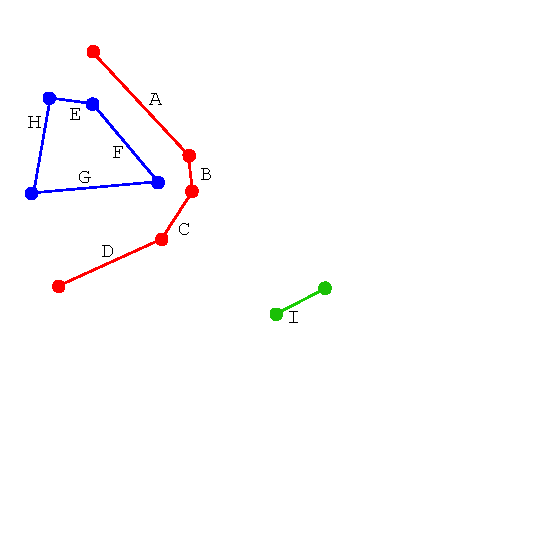
\includegraphics[width=0.24\columnwidth]{conflict-find-1.pdf} }
  \subfloat[][]{
    \label{fig:conflict-find-2}
    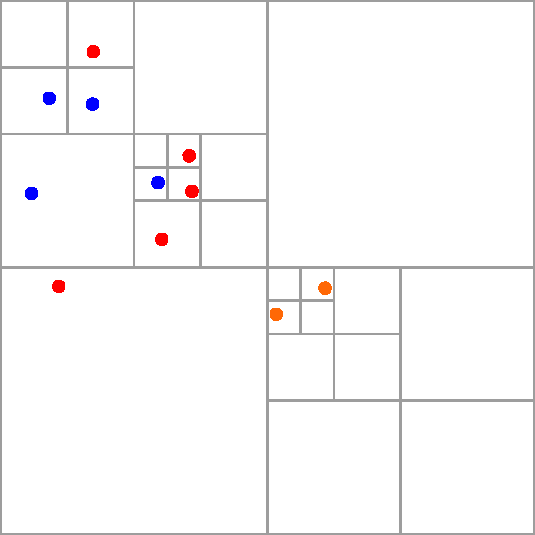
\includegraphics[width=0.24\columnwidth]{conflict-find-2.pdf} }
  \subfloat[][]{
    \label{fig:conflict-find-4}
    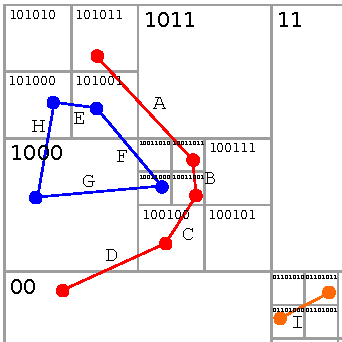
\includegraphics[width=0.24\columnwidth]{conflict-find-4.pdf} }
  \subfloat[][]{
    \label{fig:conflict-find-5}
    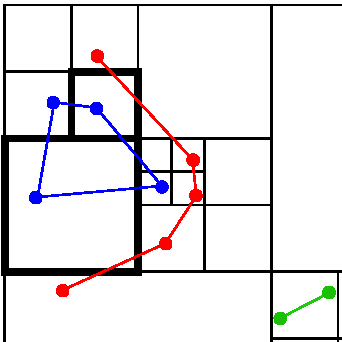
\includegraphics[width=0.24\columnwidth]{conflict-find-5.pdf} } \\
  \subfloat[][]{
    \label{fig:conflict-find-6}
    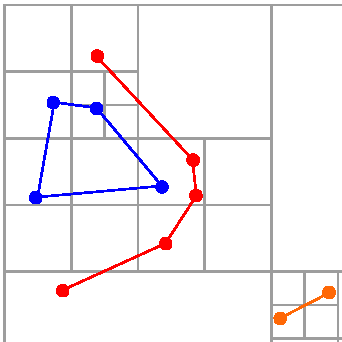
\includegraphics[width=0.24\columnwidth]{conflict-find-6.pdf} }
  \subfloat[][]{
    \label{fig:scc-sort-1}
  \begin{minipage}{0.24\columnwidth}
    \centering
    raw \\
    \vspace{0.1cm}
    \begin{tabular}{|l|l|}
      \hline
      facet & SCC \\
      \hline
      A & 10 \\
      B & 100110 \\
      C & 1001 \\
      D &  \\
      E & 1010 \\
      F & 10 \\
      G & 10 \\
      H & 10 \\
      I & 011010 \\
      \hline
    \end{tabular}
  \end{minipage} }
  \subfloat[][]{
    \label{fig:scc-sort-2}
  \begin{minipage}{0.24\columnwidth}
    \centering
    lexsort \\
    \vspace{0.1cm}
    \begin{tabular}{|l|l|}
      \hline
      facet & SCC \\
      \hline
      D &  \\
      I & 011010 \\
      A & 10 \\
      F & 10 \\
      G & 10 \\
      H & 10 \\
      C & 1001 \\
      B & 100110 \\
      E & 1010 \\
      \hline
    \end{tabular}
  \end{minipage} }
  \subfloat[][]{
    \label{fig:scc-sort-3}
  \begin{minipage}{0.24\columnwidth}
    \centering
    lensort \\
    \vspace{0.1cm}
    \begin{tabular}{|l|l|}
      \hline
      facet & SCC \\
      \hline
      D &  \\
      A & 10 \\
      F & 10 \\
      G & 10 \\
      H & 10 \\
      C & 1001 \\
      E & 1010 \\
      I & 011010 \\
      B & 100110 \\
      \hline
    \end{tabular}
  \end{minipage} }
  \caption{
    \protect\subref{fig:conflict-find-1} We have three objects, blue, red, and orange with facets labeled A-I.
    \protect\subref{fig:conflict-find-2} We construct an initial quadtree on the vertices using Karras' algorithm.
    \protect\subref{fig:conflict-find-4} We then compute the smallest common cell (SCC) for each facet. These pairs are given in figure \protect\subref{fig:scc-sort-1}.
    \protect\subref{fig:conflict-find-5} Conflict cells, which intersect more than one object, are highlighted.
    \protect\subref{fig:conflict-find-6} The new quadtree after conflict resolution.
    \protect\subref{fig:scc-sort-1} The SCC-facet pairs are stored in an array initially sorted on facet index (letters are used here for clarity). We then sort the pairs using two stable, parallel radix sorts on SCC address for fast indexed access.
    The first sort is \textit{lexsort}, a lexicographical sort \protect\subref{fig:scc-sort-2},
    then comes \textit{lensort}, a sort by length \protect\subref{fig:scc-sort-3}. In the \textit{lexsort}, we implicitly pad with zeros on the right so that all values are the same length. \red{How exactly is the \textit{lensort} done?}
  }
  \label{fig:conflict-find}
\end{figure}

\begin{figure}
  \label{fig:scc-sort}
\end{figure}

Then we use the SCC array to find the conflict cells using algorithm \ref{alg:find-conflict-cells}.

\algorithmspace
\begin{algorithm}
  \DontPrintSemicolon
  \LinesNumbered
  \KwIn{VertexQuadtree}
  \BlankLine
  \ForPar{leaf cell $L$}{
    $L$.color = -1\;
    \ForEach{cell $A$ in \directAncestors{$L$}}{
      id := compute\_cell\_index($A$)\;
      \ForEach{cell2facet in identical elements of cells2facets[id]}{
        $f$ := cell2facet.facet\;
        \If{$f$ intersects $L$}{
          \If{$L$.color == -1} {
            \tcp{First facet found}
            \tcp{that intersects $L$}
            $L$.color = $f$.color\;
            $L$.facet[0] = $f$\;
          }
          \ElseIf{$L$.color != $f$.color} {
            \tcp{Cell $L$ is ambiguous}
            $L$.color = -2\;
            $L$.facet[1] = $f$\;
          }
        }
      }
    }
  } \label{alg:quadtree_intersections_end}
\caption{FIND\_CONFLICT\_CELLS}
\label{alg:find-conflict-cells}
\end{algorithm}
\algorithmspace

\subsection{Resolve conflict cells}

%\begin{adjustbox}{valign=t}
\begin{figure}
  \centering
  \subfloat[][]{
    \label{fig:conflict-resolution-x}
    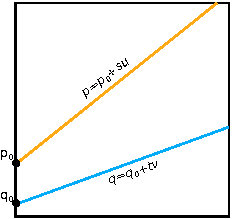
\includegraphics[width=0.24\columnwidth]{conflict-resolution-x.pdf} }
  \subfloat[][]{
    \label{fig:conflict-resolution-even}
    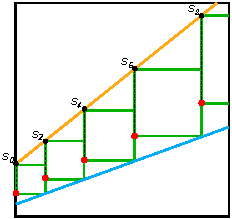
\includegraphics[width=0.24\columnwidth]{conflict-resolution-even.pdf} }
  \subfloat[][]{
    \label{fig:conflict-resolution-all}
    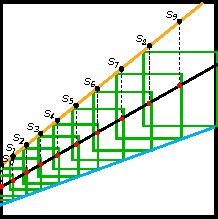
\includegraphics[width=0.24\columnwidth]{conflict-resolution-all.pdf} }
  \subfloat[][]{
    \label{fig:conflict-resolution-octree}
    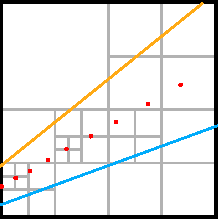
\includegraphics[width=0.24\columnwidth]{conflict-resolution-octree.pdf} } \\
  \subfloat[][]{
    \label{fig:conflict-resolution-adjacent-even}
    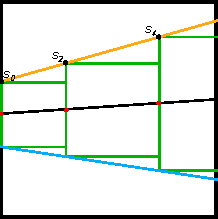
\includegraphics[width=0.24\columnwidth]{conflict-resolution-adjacent-even.pdf} }
  \subfloat[][]{
    \label{fig:conflict-resolution-adjacent-all}
    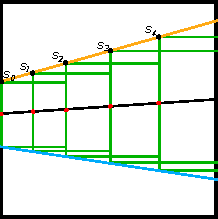
\includegraphics[width=0.24\columnwidth]{conflict-resolution-adjacent-all.pdf} }
  \caption{
    \protect\subref{fig:conflict-resolution-x} A conflict cell with two lines from different objects.
    \protect\subref{fig:conflict-resolution-even} Fitting boxes such that any box intersecting both lines contains at least one sample (red dots).
    \protect\subref{fig:conflict-resolution-even} Fitting boxes such that any box intersecting both lines contains at least two samples. This ensures that an quadtree built from the samples using Karras' algorithm (panel \protect\subref{fig:conflict-resolution-octree}) will have no leaf cells that intersect both lines, ensuring that the new quadtree is locally free of conflict cells.
  }
  \label{fig:conflict-resolution}
\end{figure}
%    \end{adjustbox}


%\begin{equation}
%\label{eqn:p}
%p(s) = p = p_0 + su
%\end{equation}
%\begin{equation}
%\label{eqn:q}
%q(s) = q = q_0 + tv
%\end{equation}
%\begin{equation}
%\label{eqn:a_}
%a(s) = a = |p^x-q^x| = |p^y-q^y|
%\end{equation}

A conflict cell is a quadtree cell that intersects at least two different objects. To resolve a conflict cell $c$, we consider pairs of lines of differing labels that intersect $c$. Figure \ref{fig:conflict-resolution-x} shows two lines

\begin{align}
q(t) &= q = q_0 + tv \label{eqn:q} \\
r(f) &= r = r_0 + fw \label{eqn:r}
\end{align}
along with a line
\begin{align}
p(s) &= p = p_0 + su \label{eqn:p}
\end{align}
that bisects $q$ and $r$. Our strategy will be to sample points $P$ on $p(s)$ (figure \ref{fig:conflict-resolution-octree}) such that an quadtree built on $V \cup P$ will completely ``separate'' $q$ and $r$, i.e., no descendent cell of $c$ will intersect both $q$ and $r$. We do this by ensuring that $P$ is sampled such that every box that intersects both $q$ and $r$ also intersects at least two points in $P$. Because Karras' algorithm guarantees that every leaf cell intersects at most one point, we know that no leaf cell will intersect $q$ and $r$ and thus no leaf cell will be a conflict cell. We will find a series of boxes such that each box's left-most intersection with $p(s)$ is a sample point meeting the above criterion.

We consider only cases where the slope of $p$ is in the range $0 \le m \le 1$. All other cases can be transformed to this case using rotation and reflection. We begin by fitting the smallest box centered on a point $p$ that intersects both $q$ and $r$. We break the problem into two cases: the \textit{opposite} case (see Figure \ref{fig:conflict-resolution-even}) is where $w^y > 0$, so each box intersects $q$ and $r$ at its top-left and bottom-right corners, respectively. The \textit{adjacent} case (see Figure \ref{fig:conflict-resolution-adjacent-even}) is where $w^y < 0$, so the line intersections are adjacent at the top-left and bottom-left corners of the box.

\subsubsection{Finding $a(s)$ -- \textit{opposite} case}

Given a point $p(s)$, we wish to find $a=a(s)$, which will give us the starting $x$ coordinate for the next box. Consider the top-left corner of the box $q(t(s))=q(t)$ and the bottom-right corner $r(f(s))=r(f)$.

Because $p^x(s)=q^x(t)$,
\begin{equation}
t = \frac{p^x(s)-q_0^x}{v^x} = \frac{p_x^x-q_0^x+su^x}{v^x} \label{eqn:t}
\end{equation}
Because our boxes are square,
\begin{equation}
r(f) = r_0+fw = q_0+tv+a\begin{bmatrix}1\\-1\end{bmatrix} \label{eqn:ro}
\end{equation}
From \eqref{eqn:ro},
\begin{align}
f &= \frac{1}{w^y}(q_0^y+tv^y-a-r_0^y) \label{eqn:f} \\
a &= r_0^x+fw^x-q_0^x-tv^x \label{eqn:a1o}
\end{align}
Substituting equations \eqref{eqn:t} and \eqref{eqn:f} into equation \eqref{eqn:a1o} and solving for $a$,
\begin{equation}
a(s) = \hat{\alpha}_o s + \hat{\beta}_o \label{eqn:ao}
\end{equation}
where
\begin{equation}
\hat{\alpha}_o = \frac{u^x|w \times v|}{v^x(w^x+w^y)}
\end{equation}
and
\begin{equation}
\hat{\beta}_o = \frac{|w \times v|(p_0^x-q_0^x) + v^x(|r_0 \times w| + |w \times q_0|)}{v^x(w^x+w^y)}
\end{equation}

\subsubsection{Finding $a(s)$ -- \textit{adjacent} case}

Consider the top-left corner of the box $q(t(s))=q(t)$ and the bottom-left corner $r(f(s))=r(f)$. $r(f)$ is now defined as
\begin{equation}
r(f) = r_0+fw = q_0+tv+a\begin{bmatrix}0\\-1\end{bmatrix} \label{eqn:ra}
\end{equation}
Equations \eqref{eqn:t} and \eqref{eqn:f} remain the same while \eqref{eqn:a1o} becomes
\begin{equation}
0 = r_0^x+fw^x-q_0^x-tv^x \label{eqn:a1a}
\end{equation}
Substituting equations \eqref{eqn:t} and \eqref{eqn:f} into equation \eqref{eqn:a1a} and solving for $a$,
\begin{equation}
a(s) = \hat{\alpha}_a s + \hat{\beta}_a \label{eqn:aa}
\end{equation}
where
\begin{equation}
\hat{\alpha}_a = \frac{u^x}{v^xw^x}
\end{equation}
and
\begin{equation}
\hat{\beta}_a = \frac{w^x(p_0^x-q_0^x)+|w \times q_0| + |r_0 \times w|}{w^x}
\end{equation}


%
%
%Because $p^x(s)=q^x(t)$,
%\begin{equation}
%t = \frac{p^x(s)-q_0^x}{v^x} = \frac{p_x^x-q_0^x+su^x}{v^x} \label{eqn:t}
%\end{equation}
%Because our boxes are square,
%\begin{equation}
%r(f) = r_0+fw = q_0+tv+a
%\begin{bmatrix}
%1\\-1
%\end{bmatrix}
%\label{eqn:r}
%\end{equation}
%From \eqref{eqn:r},
%\begin{align}
%f &= \frac{1}{w^y}(q_0^y+tv^y-a-r_0^y) \label{eqn:f} \\
%a &= r_0^x+fw^x-q_0^x-tv^x \label{eqn:a1}
%\end{align}
%Substituting equations \eqref{eqn:t} and \eqref{eqn:f} into equation \eqref{eqn:a1} and solving for $a$,
%\begin{equation}
%a = \alpha s + \beta
%\end{equation}
%where
%\begin{equation}
%\alpha = \frac{u^x|w \times v|}{v^x(w^x+w^y)}
%\end{equation}
%and
%\begin{equation}
%\beta = \frac{|w \times v|(p_0^x-q_0^x) + v^x(|r_0 \times w| + |w \times q_0|)}{v^x(w^x+w^y)}
%\end{equation}
%
%Consider a box with edge length $a_0$ centered on a point $p_0 \in p$. We first find $p$, which is the line that is equidistant from $q$ and $r$ along the diagonal vector $\gamma = (1, -1)$. Given some point $q(t)$,
%\begin{equation}
%q_0+tv + \lambda\gamma = r_0+fw \\
%\end{equation}
%Solving for $\lambda$,
%\begin{align}
%f &= \frac{1}{w^y}(q_0^y+tv^x-\lambda-r_0^y) \\
%\lambda &= r_0^x + fw^x-q_0^x-tv^x \\
%        &= r_0^x+\frac{w^x}{w^y}(q_0^y+tv^y-\lambda-r_0^y) - q_0^x-tv^x \\
%        &= \frac{1}{w^x+w^y}(r_0^xw^y+q_0^yw^x-r_0^yw^x-q_0^xw^y+t(v^yw^x-v^xw^y)
%\end{align}
%The vector $u = p - p_0$. We obtain $p$ from $q(0)$, by finding $\lambda/2$.
%\begin{align}
%p = q(0) + \frac{\lambda}{2}\gamma
%\end{align}
%We get $p_0$ by finding the intersection between the two lines. If they are parallel then we find two points $p$ using $q(0)$ and $q(1)$.
%
%To find $a$,
%\begin{align} 
%p^x-\frac{a}{2} &= q^x \\
%p^y+\frac{a}{2} &= q^y
%\end{align}
%Substituting equation \eqref{eqn:q},
%\begin{align} 
%t = \frac{p^x-a/2-q_0^x}{v^x} \\
%t = \frac{p^y+a/2-q_0^y}{v^y}
%\end{align}
%which leads to
%\begin{align} 
%\frac{p^x-a/2-q_0^x}{v^x} &= \frac{p^y+a/2-q_0^y}{v^y}
%\end{align}
%Solving for $a$,
%\begin{align}
%\label{eqn:plain_a}
%a &= \frac{2(p^xv^y-q_0^xv^y-p^yv^x+q_0^yv^x)}{v^x+v^y}
%\end{align}
%$a$ is a parametric function in $s$, so using equations \eqref{eqn:plain_a} and \eqref{eqn:p},
%\begin{align}
%a(s) &= \frac{2((p_0^x+su^x)v^y-q_0^xv^y-(p_0^y+su^y)v^x+q_0^yv^x)}{v^x+v^y} \\
%     &= s\frac{2(u^xv^y-u^yv^x)}{v^x+v^y} + \frac{2(p_0^xv^y-q_0^xv^y-p_0^yv^x+q_0^yv^x)}{v^x+v^y} \label{eqn:a}
%\end{align}
%Figure \ref{fig:conflict-resolution-even} shows that we will find a series of points $P=p(s_i)$ such that
%\begin{equation}
%p^x(s_i) = p^x(s_{i-2})+a(s_{i-2}) \label{eqn:p_s}
%\end{equation}
%Using equations \eqref{eqn:p}, \eqref{eqn:a} and \eqref{eqn:p_s},
%\begin{align}
%p_0^x+s_iu^x = p_0^x+s_{i-2}u^x+s_{i-2}\frac{2(u^xv^y-u^yv^x)}{v^x+v^y} + \frac{2(p_0^xv^y-q_0^xv^y-p_0^yv^x+q_0^yv^x)}{v^x+v^y}
%\end{align}
%Solving for $s_i$,
%\begin{equation}
%\label{eqn:si_rec}
%s_i = s_{i-2}\alpha + \beta
%\end{equation}
%where
%\begin{align}
%%\alpha &= \frac{u^xv^x+3u^xv^y-2u^yv^x}{u^x(v^x+v^y)}
%\alpha &= 1+\frac{2(u^xv^y-u^yv^x)}{u^x(v^x+v^y)} \\
%\beta &= \frac{2(p_0^xv^y-q_0^xv^y-p_0^yv^x+q_0^yv^x)}{u^x(v^x+v^y)}
%\end{align}

\subsubsection{Sampling}
In both the \textit{opposite} and the \textit{adjacent} cases, $a(s)$ is of the form $a(s) = \hat{\alpha} s + \hat{\beta}$. We now use $a(s)$ to construct a sequence of $s$ values $S = \{s_0, s_1, s_2, \dots, s_n\}$ that meet our sampling criterion. We first construct the even samples (see Figures \ref{fig:conflict-resolution-even} and \ref{fig:conflict-resolution-adjacent-even}). Given a starting point $p(s_0)$,
\begin{equation}
p^x(s_{i+2}) = p^x(s_i) + a(s_i)
\end{equation}
Substituting in equations \eqref{eqn:p} and \eqref{eqn:ao}/\eqref{eqn:aa},
\begin{equation}
p_0^x + s_{i+2}u^x = p_0^x + s_i + \hat{\alpha} s_i + \hat{\beta}
\end{equation}
Solving for $s_{i+2}$ gives the recurrence relation
\begin{equation}
s_{i+2} = \alpha s_i + \beta \label{eqn:recurrence}
\end{equation}
where
\begin{equation}
\alpha = 1 + \frac{\hat{\alpha}}{u^x}
\end{equation}
and
\begin{equation}
\beta = \frac{\hat{\beta}}{u^x}
\end{equation}

Constructing the odd samples is identical, except that we start at
\begin{equation}
s_1 = \left(1+\frac{\hat{\alpha}}{2u^x}\right)s_0 + \frac{\hat{\beta}}{2}
\end{equation}
which is the point in the center of the first box in the x-dimension.

We solve the recurrence relation \eqref{eqn:recurrence} using the characteristic polynomial to yield
\begin{equation}
s_i = k_1 + k_2 \alpha^i
\end{equation}
where
\begin{align}
k_1^{even} &= \frac{\beta}{1-\alpha} \\
k_1^{odd} &= \frac{\beta}{1-\alpha} \\
k_2^{even} &= \frac{\alpha s_0 + \beta - s_0}{\alpha-1} \\
k_2^{odd} &= \frac{\alpha s_1 + \beta - s_1}{\alpha-1}
\end{align}
The last step to formulating $P$ for parallel computation is to determine how many samples we will need. Let $p(s_{exit})$ be the point at which the line $p$ exits the cell.
\begin{align}
k_1+k_2\alpha^i < s_{exit}
\end{align}
results in
\begin{align}
i < \log_{\alpha}\frac{s_{exit}-k_1}{k_2}
\end{align}

%
%. When $i$ is odd, the initial condition will be where $s$ is halfway along the first box (it could be anywhere in the interior of the first box, but we use halfway for convenience). So from \eqref{eqn:p},
%\begin{align}
%s_1 &= \frac{p^x-p_0^x}{2u^x} \\
%    &= \frac{a(0)}{2u^x}
%\end{align}
%\begin{align}
%k_1^{even} = k_1^{odd} &= \beta\left(1-\frac{\alpha}{\alpha-1}\right) \\
%k_2^{even} &= \frac{\beta}{\alpha-1} \\
%k_2^{odd} &= \frac{a(0)}{2u^x}+\frac{\beta}{\alpha-1}
%\end{align}
%
%It is tempting to formulate the recurrance relation using a single initial condition. This would be done by replacing equation \eqref{eqn:xi_init} with
%\begin{align}
%x_i &= x_{i-1} + \frac{a(s_{i-1})}{2}
%\end{align}
%This formulation can lead to conflict cells as shown in figure \ref{fig:conflict-resolution-half}.
%
%\begin{figure}
%  \centering
%  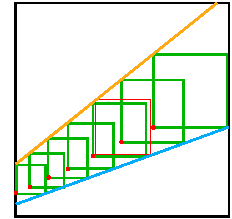
\includegraphics[width=0.48\columnwidth]{conflict-resolution-half.pdf}
%  \caption{Using a single recurrence solution we can no longer guarantee that every box that intersects both lines contains at least two samples. The box in red contains only one sample, so the quadtree may contain conflict cells.
%  }
%  \label{fig:conflict-resolution-half}
%\end{figure}



%With $a$ in hand, the question becomes, at what value of $s$ does $a(s)$ double? We desire to build a sequence $S=(s_0, s_1, \dots)$ such that $a(s_i) = 2a(s_{i-1})$. Substituting \eqref{eqn:p} into \eqref{eqn:a_prime} we get
%\begin{align}
%\label{eqn:klm}
%2a(s_{i-1}) &= \frac{q_0^xv^y-q_0^yv^x+(p_0^y+s_iu^y)v^x-(p_0^x+s_iu^x)v^y}{v^x+v^y} \nonumber \\
%&= \frac{q_0^xv^y-q_0^yv^x+p_0^yv^x-p_0^xv^y+s_i(u^yv^x-u^xv^y)}{v^x+v^y}
%\end{align}
%Solving for $s_i$ results in
%\begin{equation}
%\label{eqn:klm}
%s_i = \frac{2(v^x+v^y)a(s_{i-1})-q_0^xv^y+q_0^yv^x-p_0^yv^x+p_0^xv^y}{u^yv^x-u^xv^y}
%\end{equation}
%
%For $i>0$, $a(s_i)=a'(s_i)$, so we can characterize $s_i$ as a linear equation:
%\begin{align}
%s_0 &= 0 \nonumber \\
%s_1 &= 2ma(s_0)+b \nonumber \\
%s_2 &= 2^2ma(s_0)+b \nonumber \\
%\cdots \nonumber \\
%s_i &= 2^ima(s_0)+b
%\label{eqn:si}
%\end{align}
%where 
%\[m=\frac{v^x+v^y}{u^yv^x-u^xv^y}\]
%and
%\[b=\frac{-q_0^xv^y+q_0^yv^x-p_0^yv^x+p_0^xv^y}{u^yv^x-u^xv^y}\]
%%where $m=(v^x+v^y)/(u^yv^x-u^xv^y)$ and $b=(-q_0^xv^y+q_0^yv^x-p_0^yv^x+p_0^xv^y)/(u^yv^x-u^xv^y)$.
%
%The number of elements in sequence $S$ is obtained by setting equation \eqref{eqn:si} less than one and solving for $i$:
%\begin{equation}
%i < \log_2{\frac{1-b}{ma(s_0)}}
%\end{equation}

\subsection{Build quadtree on vertices}

We first construct an quadtree on the vertices of the objects, which we call the ``vertex quadtree''. We use Karras' algorithm \cite{karras2012maximizing} which sorts the Morton codes of the vertices in parallel, then constructs the binary radix tree in parallel. With the binary radix tree, the quadtree can be constructed with a single parallel call. The strength of this algorithm lies in the fact that overall performance scales linearly with the number of cores, regardless of the distribution of points. That is, even if a large number of vertices are clustered in a small area, requiring deep quadtree subdivision, only a constant number of parallel calls need be made. Given enough parallel units, the Karras algorithm runs in $O(\log{N})$ time, where $N$ is the number of vertices.

\subsection{Identify conflict cells}

Our end goal is to construct an quadtree such that no quadtree cell intersects more than one object. Note that a cell is allowed to intersect more than one facet, but all facets must belong to the same object, or, in other words, all facets must share the same label. It is possible, but unlikely, that the vertex quadtree has this property. If so, then we are done. Otherwise, we must identify subdivide conflict cells.

One naive algorithm to identify conflict cells is to process each leaf cell $c$ in parallel and store which facets intersect $c$. This is $O(N)$. Another approach is to process each facet in parallel and add it to every cell that it intersects. This is $O(k\log{N})$ where $k$ is maximum number of cells that any facet intersects. As we will show, our algorithm is $O(j + \log{N})$ where $j$ is the maximum number of facets that intersect any cell. In practice, $\log{N} > j$, making our algorithm $O(\log{N})$.

We identify conflict cells as shown in algorithm \ref{alg:find-conflict-cells}. In lines \ref{alg:quadtree_containing_begin}-\ref{alg:quadtree_containing_end}, for each internal quadtree cell $c$, we store all facets for which $c$ is the smallest containing cell. Since we are implementing this in a GPGPU environment, we don't have dynamic memory, so each facet must be processed twice. The first loop discovers how many facets are to be stored in each cell after which we allocate space for the facets. We use parallel prefix sums to determine the amount of space we need to allocate as well as the offsets for each internal cell. The second loop actually stores the facets.

The $\container{f}$ procedure finds the smallest quadtree cell that fully contains the facet $f$. A straightforward implementation of $\container{f}$ is to perform a standard quadtree search on the vertices of $f$ and take the smallest quadtree cell that contains all of them. (Note that the cell is always an internal node, since a post-condition of the Karras algorithm is that no leaf cell contains more than one vertex.) In our implementation however, we take advantage of our existing data structures. The quadtree cell that contains a vertex $v$ is uniquely determined by the D-tuple bits of its morton code. For example, if a 2D vertex has morton code $010010$, then the quadtree is traversed from the root to child $01$ to child $00$ to child $10$. To determine $\container{f}$, we find the longest common prefix (\lcp) of the vertices. Truncating the length of \lcp\,to a multiple of D, we find the smallest quadtree cell that contains all vertices of $f$. The complexity of $\container{f}$ is $O(\log{N})$ for both implementations. Thus, lines \ref{alg:quadtree_containing_begin}-\ref{alg:quadtree_containing_end} run in $O(\log{N})$ time.

Lines \ref{alg:quadtree_intersections_begin}-\ref{alg:quadtree_intersections_end} of the algorithm identify and store all facets that intersect with a given leaf cell $c$. Again, it is done in two steps for memory allocation purposes. Each leaf cell $c$ looks at its $O(\log{N})$ ancestors and tests all facets stored in those ancestors for intersection with $c$. Any intersecting facets get stored in $c$. These lines run in $O(F)$ time, where $F$ is the number of facets in all objects. Even though the loop is doubly-nested, each facet is stored in a unique internal node, so no more than $F$ facets will be visited in the loops. In practice, far fewer than $F$ facets will be checked for each leaf cell, because most datasets have facets that are completely contained in internal cells that are reasonably low in the tree.

The entire conflict cell detection algorithm runs in $O(\log{N}+L) = O(L)$ because $L > \log{N}$. However, average case is $O(\log{N})$, considering that most lines are contained entirely in a cell at reasonably low depth.

In Step 4, Stack is preallocated to size $M\cdot2^D$ where $M$ is the maximum quadtree depth and $D$ is the dimension. A conflict cell is a cell that intersects at least two different objects, or two lines of different labels.


The second procedure we use is $\directAncestors{c}$, which finds all ancestors of quadtree cell $c$.


%\SetKwFor{ForPar}{for}{do in parallel}{endfpar}

\algorithmspace
\begin{algorithm}
  \DontPrintSemicolon
  \LinesNumbered
  \KwIn{VertexQuadtree}
  \BlankLine
  \tcp{Store contained facets}
  \ForPar{facet $f$ in Objects}{
    \label{alg:quadtree_containing_begin}
    a := $\container{f}$\;
    a.numFacets := a.numFacets + 1\;
  }
  Allocate space for facets in internal cells\;
  \ForPar{facet $f$ in Objects}{
    a := $\container{f}$\;
    a.facets := a.facets $\cup$ f
  } \label{alg:quadtree_containing_end}
  \tcp{Store intersecting facets}
  \ForPar{leaf cell c in VertexQuadtree}{
    \label{alg:quadtree_intersections_begin}
    \ForEach{cell a in \directAncestors{c}}{
      \ForEach{facet $f$ in a.facets}{
        \If{$f$ intersects c}{
          c.numFacets := c.numFacets + 1\;
        }
      }
    }
  }
  Allocate space for facets in leaf cells\;
  \ForPar{leaf cell c in VertexQuadtree}{
    \ForEach{cell a in \directAncestors{c}}{
      \ForEach{facet $f$ in a.facets}{
        \If{$f$ intersects c}{
          c.facets := c.facets $\cup$ f\;
        }
      }
    }
  } \label{alg:quadtree_intersections_end}
\caption{FIND\_CONFLICT\_CELLS}
\label{alg:find-conflict-cells}
\end{algorithm}
\algorithmspace

\algorithmspace
\begin{algorithm}
  \DontPrintSemicolon
  \LinesNumbered
  \KwIn{Quadtree, conflict\_cells}
  \BlankLine
  \tcp{4. Quadtree refinement}
  \ForPar{leaf cell c in Quadtree}{
    c' := c\;
    \While{c' $\in$ conflict\_cells}{
      $(c'_0,c'_1,\dots,c'_{2^D-1})$ := subdivide c'\;
      push $(c'_0,c'_1,\dots,c'_{2^D-1})$ onto Stack\;
      c' := Stack.pop
    }
  }
\caption{REFINE\_QUADTREE}
\label{alg:refine-quadtree}
\end{algorithm}
\algorithmspace

\begin{figure}
  \centering
  \subfloat[][]{
    \label{fig:octree-cartesian-1}
    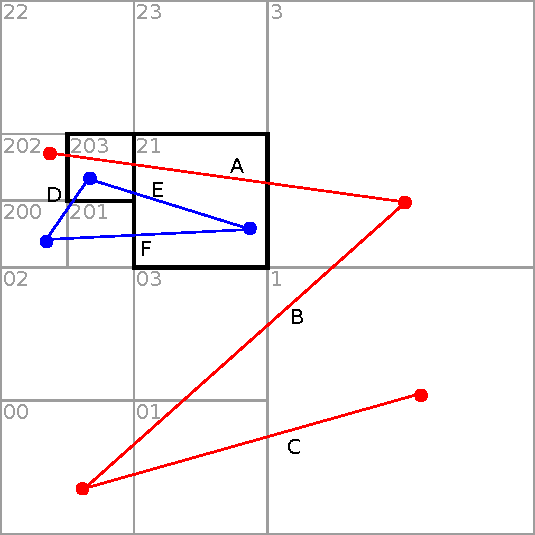
\includegraphics[width=0.24\columnwidth]{octree-cartesian-1.pdf} }
  \subfloat[][]{
    \label{fig:octree-cartesian-2}
    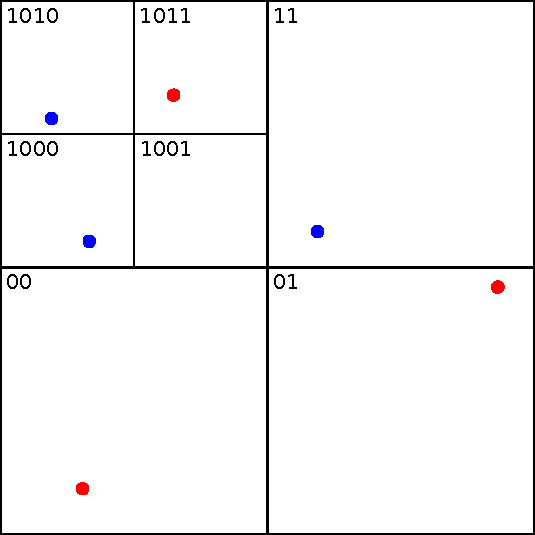
\includegraphics[width=0.24\columnwidth]{octree-cartesian-2.pdf} }
  \subfloat[][]{
    \label{fig:octree-cartesian-3}
    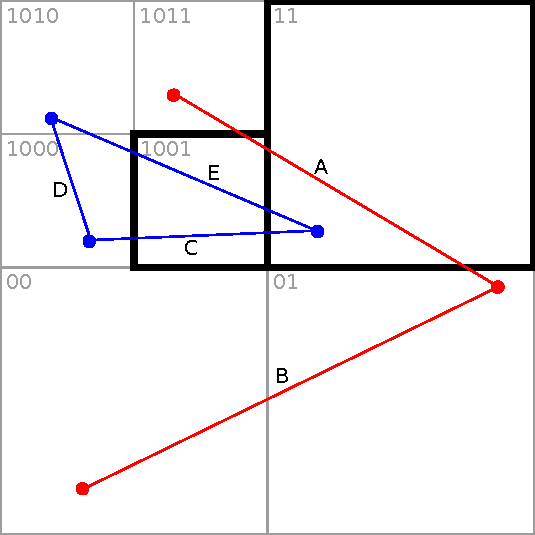
\includegraphics[width=0.24\columnwidth]{octree-cartesian-3.pdf} }
  \subfloat[][]{
    \label{fig:octree-cartesian-5}
    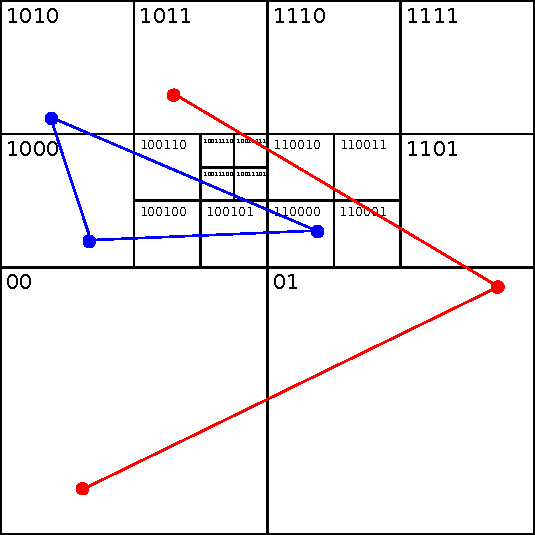
\includegraphics[width=0.24\columnwidth]{octree-cartesian-5.pdf} } \\
  \subfloat[][]{
    \label{fig:octree-hierarchical-1}
    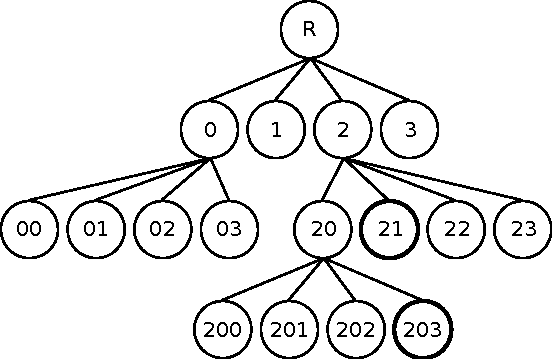
\includegraphics[width=0.24\columnwidth]{octree-hierarchical-1.pdf} }
  \subfloat[][]{
    \label{fig:octree-hierarchical-2}
    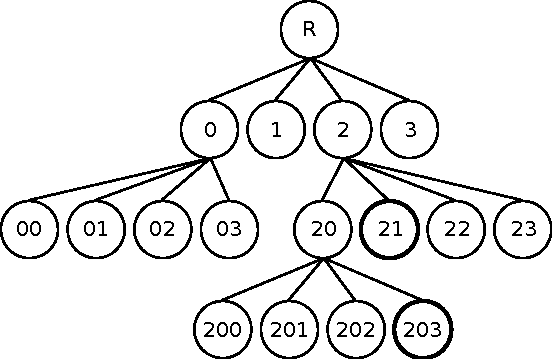
\includegraphics[width=0.24\columnwidth]{octree-hierarchical-2.pdf} }
  \caption{
    \protect\subref{fig:octree-cartesian-1} A red object and a blue object.
    \protect\subref{fig:octree-cartesian-2} The vertex quadtree, or quadtree built on the object vertices using Karras' algorithm.
    \protect\subref{fig:octree-cartesian-3}, \protect\subref{fig:octree-hierarchical-1} The vertex quadtree with conflict cells highlighted. Note the label of an quadtree cell in \protect\subref{fig:octree-cartesian-3} is the concatenation of labels from root R to the leaf cell in \protect\subref{fig:octree-hierarchical-1}. This value also corresponds to the highest order bits of the morton code of any point in the cell.
    \protect\subref{fig:octree-cartesian-5}, \protect\subref{fig:octree-hierarchical-2} The quadtree after resolution of conflict cells.
  }
  \label{fig:steps}
\end{figure}

In Fig. \ref{fig:steps}, R (Root) is the smallest containing cell for lines A, B, and C, cell 20 contains line D, and cell 2 contains lines E and F. After Step 3 of the algorithm, line A is stored in leaf cells 202, 203, 21, and 3. Conflict cells, which are the only cells that are subdivided, are 203 and 21.

%\begin{table}
%  \centering
%  \begin{tabular}{ll}
%    \toprule
%    line &  $\container{line}$ \\
%    \midrule
%    A & R \\
%    B & R \\
%    C & R \\
%    D & 20 \\
%    E & 2 \\
%    F & 2 \\
%    \bottomrule
%  \end{tabular}
%\end{table}


%-----------------------------------------------------------
% Compute GVD surface
%-----------------------------------------------------------
\section{Compute GVD surface}
\label{sec:bisector}

%-------------------------------------------------------------------------------
% Results
%-------------------------------------------------------------------------------
\section{Results and applications}
Our implementation\footnote{Source code is available at \url{http://cedmav.org/research/project/33-gvds.html}.} of the algorithm supports \red{polygons and} triangulated objects, and our wavefront initialization step is implemented on the GPU using OpenCL. All tests were run on a MacBook Pro laptop with a dual-core 2.9 GHz processor, 8 GB memory, and Intel HD 4000 graphics card. Figure \ref{fig:bunny} shows our implementation of the GVD computation pipeline, and Figure \ref{fig:pipes} shows the computed GVD on a more challenging dataset.  We compare our method with other work and then show examples in three application settings: path planning, proximity queries, and exploded diagrams.

\subsection{Comparison to other methods}


% # quadtree vertices
%  52K ./viewer3 -l 8 ~/data/gears/gear[1-3].obj
% 170K ./viewer3 -l 12 ~/data/knife/knife-holder.obj ~/data/knife/knife[2-4].obj
% 146K ./viewer2 -l 24 ../data2/filled_ut/*.dat
% 2.8M ./viewer3 --uniform-colors -a 1 -l 8 ~/data/neuron/improved/a*.obj
% 1.3M ./viewer3 -l 8 ~/data/rice-dwarf/decimated2/n1UF2a-*.obj

% memory (54 bytes per quadtree cell)
%  2.8Mb ./viewer3 -l 8 ~/data/gears/gear[1-3].obj
%  9.2Mb ./viewer3 -l 12 ~/data/knife/knife-holder.obj ~/data/knife/knife[2-4].obj
% 7.9Mb ./viewer2 -l 24 ../data2/filled_ut/*.dat
% 151.2Mb ./viewer3 --uniform-colors -a 1 -l 8 ~/data/neuron/improved/a*.obj
% 70.2Mb ./viewer3 -l 8 ~/data/rice-dwarf/decimated2/n1UF2a-*.obj

\begin{table*}
  \centering
  \footnotesize{
  \begin{tabular}{l c c c c c c c}
    \toprule
    dataset & objects & object          & quadtree   & quadtree          & quadtree &
    GVD   & GVD             \\
            &         & $\Delta$s       & depth    & cells           & memory &
    (sec) & $\Delta$s       \\
            &         & ($\times 10^3$) &          & ($\times 10^3$) & (Mb)   &
          & ($\times 10^3$) \\
    \midrule
    % ./viewer3 -l 8 ~/data/gears/gear[1-3].obj
    Fig. \ref{fig:gears} & 3 & 7 & 8 & 54 & 3 & 0.9 & 83\\
    % ./viewer3 -l 12 ~/data/knife/knife-holder.obj ~/data/knife/knife[2-4].obj
    Fig. \ref{fig:knife} & 4 & 15 & 12 & 146 & 9 & 3.9 & 232 \\
    % ./viewer2 -l 24 ../data2/filled_ut/*.dat
    Fig. \ref{fig:path} & 470 & 5 & 24 & 158 & 8 & 2.0 & 151 \\
    % ./viewer3 --uniform-colors -a 1 -l 8 ~/data/neuron/improved/a*.obj
    Fig. \ref{fig:axons} & 448 & 4015 & 8 & 2716 & 151 & 195 & 8100 \\
    % ./viewer3 -l 8 ~/data/rice-dwarf/decimated2/n1UF2a-*.obj
    Fig. \ref{fig:mol-explode} & 35 & 1500 & 8 & 496 & 70 & 19 & 2700 \\
    \bottomrule
  \end{tabular}}
  \caption{Table of quadtree/GVD computation statistics and timings on datasets that are unmanageable using other methods. \red{Columns are: \emph{objects} - the number of objects in the dataset; \emph{object $\Delta$s} - the number of line segments (2D) or triangles (3D) of all objects in the dataset; \emph{quadtree depth} - required quadtree depth in order to resolve objects; \emph{quadtree cells} - total number of leaf quadtree cells; \emph{quadtree memory} - amount of memory used by the quadtree; \emph{GVD (sec)} - seconds to perform all steps of GVD computation; \emph{GVD $\Delta$s} - number of line segments (2D) or triangles (3D) in the GVD.}}
  \label{tab:timings}
\end{table*}


%-------------------------------------------------------------------------------
% Conclusions
%-------------------------------------------------------------------------------
\section{Conclusions}

%-------------------------------------------------------------------------------
% Acknowledgements
%-------------------------------------------------------------------------------
%\section*{Acknowledgements}
%Thanks to Kristen Harris for use of the neuronal data and Jonathan Bronson for the heart data. The work of JE and VP was supported in part by NSF IIS-1314896, NSF ACI-0904631, DOE/NEUP 120341, DOE/UV-CDAT DESC0006872, DOE/Codesign P01180734, DOE/SciDAC DESC0007446, DOE/PIPER DESC0010498, and DOE/CCMSC DENA0002375. This work initiated at the University of Texas when JE, ED  and CB were supported in part by NIH contract R01-EB00487, NSF Grant OCI-1216701 and SNL contract 1439100.

%-------------------------------------------------------------------------
% Bibliography
%-------------------------------------------------------------------------

%\bibliographystyle{eg-alpha}
\bibliographystyle{eg-alpha-doi}
\balance
\bibliography{paper}

\end{document}
